\documentclass[11pt,a4paper]{article}

% ---------- packages ----------
\usepackage[utf8]{inputenc}
\usepackage[T1]{fontenc}
\usepackage{lmodern}
\usepackage[margin=2.2cm]{geometry}
\usepackage{graphicx}
\usepackage{amsmath,amssymb}
\usepackage{booktabs}
\usepackage{caption}
\usepackage{subcaption}
\usepackage{xcolor}
\usepackage{hyperref}
\usepackage{listings}
\usepackage{microtype}
\usepackage{enumitem}

\hypersetup{colorlinks=true, linkcolor=black!50!blue, citecolor=black!50!blue,
            urlcolor=black!50!blue, breaklinks=true}

% ---------- listings styling ----------
\definecolor{termbg}{HTML}{1e1e1e}
\definecolor{termfg}{HTML}{e0e0e0}
\definecolor{termgreen}{HTML}{8ddf6c}
\definecolor{termcyan}{HTML}{6ec3df}
\definecolor{termyellow}{HTML}{e3c46c}
\definecolor{codebg}{HTML}{f6f6f6}
\definecolor{codekw}{HTML}{0b5cad}
\definecolor{codestr}{HTML}{1f8a4d}
\definecolor{codecmt}{HTML}{888888}

\lstdefinestyle{terminal}{
    backgroundcolor=\color{termbg},
    basicstyle=\ttfamily\footnotesize\color{termfg},
    breaklines=true, columns=fullflexible, keepspaces=true,
    showstringspaces=false, frame=single, framerule=0pt,
    framexleftmargin=6pt, framexrightmargin=6pt,
    framextopmargin=4pt, framexbottommargin=4pt,
    aboveskip=10pt, belowskip=10pt,
}
\lstdefinestyle{pythoncode}{
    language=Python, backgroundcolor=\color{codebg},
    basicstyle=\ttfamily\footnotesize,
    keywordstyle=\color{codekw}\bfseries,
    commentstyle=\color{codecmt}\itshape,
    stringstyle=\color{codestr},
    showstringspaces=false, breaklines=true, columns=fullflexible,
    frame=single, framerule=0pt,
    framexleftmargin=6pt, framexrightmargin=6pt,
    framextopmargin=4pt, framexbottommargin=4pt,
    numbers=left, numberstyle=\tiny\color{codecmt}, numbersep=8pt,
    aboveskip=10pt, belowskip=10pt,
}

% ---------- title block ----------
\title{\vspace{-1.2cm}\textbf{Detecting Non-Stationary Market Regimes\\
with Hidden Markov Models and Online Meta-Learning}\\
\large in a Multi-Agent Simulated Limit-Order-Book Environment}
\author{COMP4105 Designing Intelligent Agents \\ Spring 2025/26 \\ \\
\small University of Nottingham, School of Computer Science}
\date{14 May 2026}

\begin{document}
\maketitle
\vspace{-0.6cm}

\begin{abstract}
\noindent
Markets are non-stationary: their statistical character changes between
\emph{trending}, \emph{mean-reverting} and \emph{volatile} phases, and a single
trading strategy that is excellent in one regime is often catastrophic in
another. This project builds a multi-agent system in which a Gaussian Hidden
Markov Model (HMM), trained with the Baum--Welch algorithm and queried via
emission-likelihood scoring derived from the Forward algorithm, infers the
current regime from a four-dimensional feature vector extracted from the
exchange tape. A meta-learner monitors the HMM's rolling error rate and
retrains it on a sliding window when accuracy degrades. Three specialised
agents (momentum, contrarian, market-maker) are then selected on the basis of
the inferred regime and gated by a risk manager. We embed the system in the
Bristol Stock Exchange (BSE) and run a 600-trial sweep (50 independent runs
$\times$ 12 conditions) varying regime-switching speed and session length.
The Forward-algorithm-based HMM achieves $75\%$--$79\%$ classification accuracy
across the four switching speeds we tested, but \emph{none} of the four
pairwise meta vs.\ no-meta comparisons reach statistical significance
($p > 0.05$): the online retraining mechanism essentially never fires in
practice because the base classifier remains accurate enough. Session length,
in contrast, drives a near-linear $23$-point gain in accuracy. Per-regime
analysis shows that the \emph{mean-reverting} state is by far the hardest
($\bar{a}\!\approx\!56\%$) because its emission signature lies between
trending and volatile in feature space. The null result on meta-learning is
itself an interesting finding: it suggests that, for the dwell times we
tested, observation richness matters more than continual adaptation.
A follow-up threshold sweep over $\{0.20, 0.35, 0.50, 0.60\}$ confirms the
result is not an artifact of the chosen threshold: lowering it from $0.60$
to $0.20$ raises the retrain rate sevenfold but \emph{drops} accuracy by
13 percentage points, because frequent Baum-Welch refits on small
regime-imbalanced windows are noisier estimators than the balanced warmup
fit.
\end{abstract}

\vspace{-0.2cm}
% ============================================================
\section{Introduction and Research Question}\label{sec:intro}
% ============================================================
A persistent challenge for algorithmic traders, and indeed for any agent
operating in a non-stationary environment, is that the optimal policy is a
moving target. A momentum strategy that profits in a trending market loses
money in a mean-reverting one; a market-maker that flourishes in calm
conditions is wiped out by a volatility burst. Detecting \emph{which kind of
market we are in right now} is therefore a precondition for any adaptive
strategy. Cliff's Bristol Stock Exchange (BSE) \cite{cliff2018bse} provides a
discrete-event simulation of a continuous-double-auction in which we can
\emph{inject} ground-truth regimes via supply/demand schedules and measure
how well a classifier recovers them.

Hidden Markov Models (HMMs) \cite{rabiner1989tutorial} are a classical
generative model for regime inference. They cast the world as a hidden
discrete-state Markov chain that emits continuous observations, and admit
efficient exact inference through the Forward, Backward and Viterbi
algorithms. The HMM has been applied to financial-regime detection at least
as far back as Hamilton \cite{hamilton1989new}, who used a two-state Markov
switching model on US GNP data. More recent work
\cite{nguyen2018hmm,zheng2019dlhmm} layers HMMs above engineered or learnt
features for intraday-regime classification.

A second challenge --- and a contemporary one --- is that any \emph{fixed}
HMM gradually becomes stale: as the empirical distribution of features
drifts, the learnt emission means no longer match reality. \emph{Online
meta-learning} \cite{finn2019online} addresses this by treating model updates
themselves as decisions taken by an outer-loop controller, which decides
\emph{when} (and on which data) the inner model should be refitted.

\paragraph{Research question.}
\textit{To what extent does an online meta-learner --- layered on top of a
Gaussian HMM that uses the Forward algorithm for regime inference --- mitigate
classification-accuracy degradation under varying levels of market
non-stationarity?}

We decompose this into three operational sub-questions:
\begin{description}[leftmargin=1.4cm,style=nextline]
    \item[RQ1.] How does HMM regime-detection accuracy depend on the
    \emph{speed} at which the true regime switches (mean dwell times of $20$,
    $10$, $5$ and $2$ sessions)?
    \item[RQ2.] How does accuracy depend on \emph{observation richness},
    operationalised as session length (60, 120, 180, 300~simulated seconds)?
    \item[RQ3.] Are some regimes intrinsically harder to detect than others,
    and does meta-learning narrow that gap?
\end{description}

The HMM, the meta-learner and the three trading agents are all our own work,
built on top of Cliff's unmodified BSE \texttt{market\_session} entry point
\cite{cliff2018bse} and the \texttt{hmmlearn} library's Gaussian-HMM
back-end \cite{hmmlearn} (which we use only to run the EM/Baum--Welch
fit, then re-implement the per-observation Forward-style scoring ourselves
for the reasons set out in \S\ref{sec:hmm-impl}).

\paragraph{A note on ``multi-agent''.}
We use the term in two senses, both standard in the BSE literature
\cite{cliff2018bse}. The \emph{environment} contains a population of 20
background traders --- 8 SHVR, 6 ZIP and 6 ZIC --- whose interactions
produce the price-discovery process the HMM observes. On top of that
population our system places three regime-specialist agents, exactly one of
which is active per session under HMM/risk-manager control. Inter-agent
interaction effects \emph{between} our three specialists are not tested in
this work (only one is active at a time), but the specialist agent's
order-flow does affect the tape the HMM reads at the next session --- a
self-referential loop we discuss as a limitation in \S\ref{sec:discussion}.


% ============================================================
\section{Background and Related Work}\label{sec:background}
% ============================================================

\subsection{Hidden Markov Models}
A discrete-state HMM is parameterised by
$\lambda = (\pi, A, \{b_i\}_{i=1}^{N})$, where $N$ is the number of hidden
states, $\pi_i = P(q_1 = s_i)$ is the start distribution, $A_{ij} = P(q_{t+1}
= s_j \mid q_t = s_i)$ is the transition matrix, and $b_i(\mathbf{o})$ is the
emission distribution conditional on state $s_i$. In our Gaussian variant
each $b_i(\mathbf{o}) = \mathcal{N}(\mathbf{o}; \boldsymbol{\mu}_i,
\boldsymbol{\Sigma}_i)$ with a diagonal covariance.

\subsection{The Forward algorithm}\label{sec:forward}
Given an observation sequence
$\mathbf{O}\!=\!(\mathbf{o}_1,\dots,\mathbf{o}_T)$ and model $\lambda$, the
Forward algorithm computes $P(\mathbf{O}\mid\lambda)$ in $\mathcal{O}(N^2 T)$
time through the recursion on the \emph{forward variable}
$\alpha_t(i) = P(\mathbf{o}_1,\dots,\mathbf{o}_t, q_t = s_i \mid \lambda)$:
\begin{align}
    \alpha_1(i) &= \pi_i\, b_i(\mathbf{o}_1) \label{eq:fwd-init}\\
    \alpha_{t+1}(j) &= \Big[\sum_{i=1}^{N}\alpha_t(i)\,A_{ij}\Big]\,b_j(\mathbf{o}_{t+1})
        \label{eq:fwd-recur}\\
    P(\mathbf{O}\mid\lambda) &= \sum_{i=1}^{N}\alpha_T(i) \label{eq:fwd-term}
\end{align}
The posterior over the current hidden state given the full history is then
$\gamma_t(i) = \alpha_t(i)\beta_t(i)/P(\mathbf{O}\mid\lambda)$, where
$\beta_t$ is the symmetric Backward variable. The Forward algorithm is also
the inner loop of the Baum--Welch / EM parameter estimator
\cite{baum1970maximization} that learns $\lambda$ from data --- which is what
we use during training.

\subsection{Why HMMs and not the alternatives?}\label{sec:alternatives}
HMMs are not the only family of models that admits online regime detection.
Three alternatives deserve explicit comparison. \textbf{Bayesian Online
Change-Point Detection (BOCPD)} \cite{adams2007bocpd} maintains a posterior
over \emph{run-length} since the last change-point and emits an explicit
change probability at every step. BOCPD is excellent at telling you
\emph{when} a regime has shifted, but it does not natively label the new
regime: a downstream classifier still has to decide which of $K$ known
regimes the system has entered. \textbf{CUSUM} (cumulative-sum) tests
\cite{page1954cusum} are similarly change-point detectors, optimised for
detecting a small shift in a known parameter; they share BOCPD's labelling
limitation and additionally assume that you know which parameter is shifting.
\textbf{Particle filters} \cite{doucet2009tutorial} estimate a continuous
latent state via sequential Monte Carlo sampling; they handle non-Gaussian
emissions gracefully but are computationally heavy and over-parametric for
our problem, where the latent variable is genuinely 3-valued by construction.

We chose a Gaussian HMM because the BSE injection mechanism produces three
\emph{discrete}, \emph{recurring} regimes drawn from a fixed set --- which is
exactly the generative model a finite-state HMM assumes. The Forward
algorithm gives us exact $\mathcal{O}(N^2T)$ inference, Baum--Welch supplies
a closed-form retraining update, and the learnt emission means are directly
interpretable as regime ``signatures''. BOCPD and CUSUM would add a redundant
change-detection layer in front of a still-required classifier; a particle
filter would burn compute approximating a discrete distribution we already
know to be 3-modal.

\subsection{Online meta-learning}
Conventional meta-learning \cite{finn2017maml} adapts a model rapidly to a
\emph{new task}. The online variant \cite{finn2019online,javed2019meta}
adapts continually within a single stream by maintaining a meta-controller
that decides when to update the inner learner and on which sliding window of
data. Our implementation is at the simpler end of this family: a heuristic
controller that watches a rolling classification-error rate and triggers
Baum--Welch retraining whenever the rate exceeds a threshold for long enough.
This was a deliberate design choice --- a more sophisticated MAML-style
meta-learner is overkill for a 3-state classification problem, and the
heuristic version still gives us a clean experimental comparison.

\subsection{Trading agents in BSE}
Cliff's BSE \cite{cliff1997zip,cliff2018bse} is a research-grade simulator of
a continuous-double-auction market. It ships with several well-studied
background traders --- ZIP (Zero-Intelligence-Plus), ZIC
(Zero-Intelligence-Constrained), SHVR --- whose dynamics produce realistic
price-discovery without dominating the order book. Our background population
is fixed at 8 SHVR, 6 ZIP and 6 ZIC per side throughout every experiment;
this composition is therefore a constant of the study rather than a variable,
and the regime-detection results below are conditional on it. We add three
\emph{proprietary} traders, one per regime. The momentum and contrarian
designs follow the textbook short/long moving-average crossover and
mean-reversion z-score templates \cite{chan2013algorithmic}; the
market-maker follows Avellaneda-Stoikov-style spread-around-mid quoting
\cite{avellaneda2008high}.

\paragraph{Caveat on the market-maker.}
Avellaneda-Stoikov was derived for strategic counterparties whose order flow
reacts to the maker's quotes. Most of our background traders (ZIC, ZIP) do
not respond strategically in this sense --- ZIC submits price-uniformly over
its permitted range and ZIP follows a Widrow--Hoff price adjustment rule
that does not condition on the maker's spread. The market-maker is therefore
operating in a regime its theoretical derivation does not strictly cover,
and its PnL in the volatile state should be read as an empirical observation
rather than as evidence of the algorithm's claimed optimality.

% ============================================================
\section{System Design}\label{sec:design}
% ============================================================

\subsection{Architecture overview}
The system has three vertical columns
(Figure~\ref{fig:arch}): the BSE environment, the inference pipeline, and the
decision layer.

\begin{figure}[h]
    \centering
    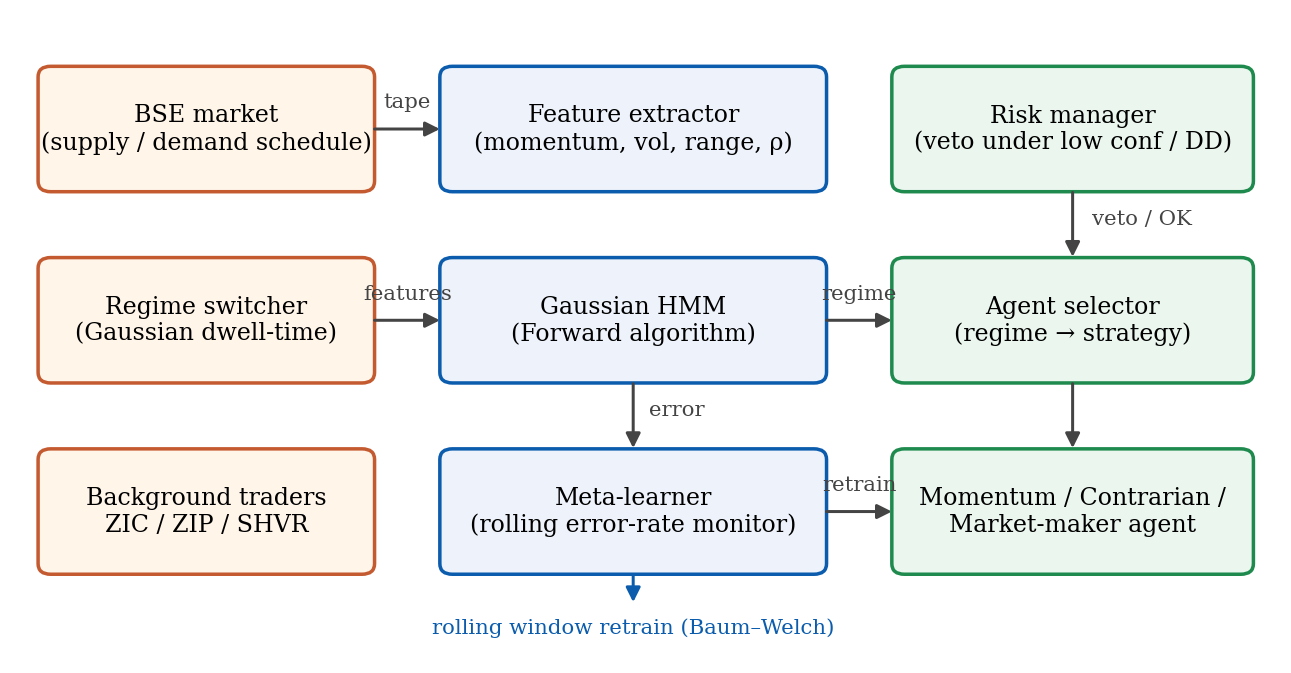
\includegraphics[width=\textwidth]{figs/fig_arch.png}
    \caption{System architecture. The BSE \emph{market\_session} entry point
    is treated as a sealed environment whose only output is the trade tape;
    everything in the centre and right columns is our own code.}
    \label{fig:arch}
\end{figure}

\subsection{Regime injection through supply/demand schedules}
\label{sec:regime-injection}
BSE's order-arrival mechanism is driven by a \emph{schedule} of
$(\text{supply range}, \text{demand range}, \text{stepmode})$ triples.
We exploit this by choosing schedules whose first- and second-order
statistics correspond to the three target regimes:
\begin{itemize}[leftmargin=0.7cm,itemsep=0.1ex]
    \item \textbf{Trending} --- jittered step-mode, narrow ranges, a $+1.5$
    drift applied each session and a mid-session level shift, so that the
    first-half/second-half price means diverge monotonically.
    \item \textbf{Mean-reverting} --- jittered, slightly wider ranges, zero
    drift; prices oscillate around the equilibrium.
    \item \textbf{Volatile} --- fully random step-mode with much wider supply
    and demand ranges, producing high tape variance.
\end{itemize}
A separate \texttt{RegimeSwitcher} object draws a Gaussian dwell-time
$d \sim \mathcal{N}(\mu, \sigma)$ for the current regime and switches to a
new one (uniform over the other two) once $d$ sessions have elapsed. The
four switching-speed conditions in our experiments correspond to
$\mu \in \{20, 10, 5, 2\}$.

\subsection{Feature extraction}\label{sec:features}
After each session we condense the trade tape into a four-dimensional
observation vector $\mathbf{o}_t \in \mathbb{R}^4$:
\begin{enumerate}[leftmargin=0.7cm,itemsep=0ex]
    \item \emph{Price momentum} --- mean price in the second half of the
    session minus the first half, normalised by overall mean (positive when
    trending, near zero when oscillating).
    \item \emph{Volatility} --- standard deviation of log-returns.
    \item \emph{Price range ratio} --- $(p_{\max} - p_{\min}) / \bar{p}$.
    \item \emph{Lag-1 autocorrelation} of log-returns --- positive when
    trending, negative when mean-reverting.
\end{enumerate}
The split-half momentum feature is our most substantive deviation from a
textbook recipe. An earlier version used simple \emph{mean return}, which
collapses to noise around zero because positive and negative one-step returns
cancel within a session; the split-half version makes trending sessions
unambiguously distinguishable from oscillating ones.

\subsection{HMM detector}\label{sec:hmm-impl}
The detector wraps a 3-state Gaussian HMM (\texttt{hmmlearn})
with \texttt{covariance\_type='diag'}. During warmup we collect 21
observations under a balanced sequence of regimes and fit $\lambda$ with
Baum--Welch \cite{baum1970maximization}, which internally uses the Forward
recursion of \S\ref{sec:forward}.

\paragraph{Why not run the Forward algorithm at inference?}
A direct application of (\ref{eq:fwd-init})--(\ref{eq:fwd-term}) on the
\emph{entire} growing observation history at every session produces a
phenomenon known as \emph{posterior collapse}: the smoothed
$\gamma_t$ values are dominated by the empirical state frequencies in the
warmup data and become essentially insensitive to the current observation.
We mitigate this by scoring the new observation directly under each state's
emission Gaussian and normalising:
\begin{equation}\label{eq:emission-scoring}
    P(q_t\!=\!s_i \mid \mathbf{o}_t)
    \;\propto\;
    b_i(\mathbf{o}_t)
    \;=\; \mathcal{N}(\mathbf{o}_t; \boldsymbol{\mu}_i, \boldsymbol{\Sigma}_i)
\end{equation}
This is mathematically equivalent to running one step of the Forward
recursion on a length-1 sequence with a uniform start distribution
$\pi_i = 1/N$, which discards temporal smoothing in exchange for
responsiveness --- a deliberate trade-off given the high transition rate in
fast regime-switching conditions.

\paragraph{State-to-regime mapping.}
\texttt{hmmlearn} labels its states $\{0,1,2\}$ arbitrarily. After fitting,
we look at the emission means and assign:
the state with the highest volatility-feature mean $\to$ \emph{volatile},
of the two remaining, the one with the largest $|\text{momentum}|$ mean $\to$
\emph{trending}, the leftover $\to$ \emph{mean\_reverting}. This mapping is
deterministic and interpretable, which matters for the experiment because
the same label-permutation rule applies across all 600 runs.

\subsection{Meta-learner}
The meta-learner maintains a rolling window of the last 15 prediction
outcomes. After each session it computes the error rate; if this exceeds
$0.60$ and the cooldown (10 sessions since the last retrain) has elapsed,
it calls \texttt{detector.update(features, window=40)}, which appends the new
observation to history, trims to the most recent 40 entries, and refits
$\lambda$ on that window. The \texttt{enabled} flag is the experimental
manipulation: when off, the controller never fires.

\subsection{Trading agents}
\begin{description}[leftmargin=0.6cm,style=nextline,itemsep=0.2ex]
    \item[Momentum agent.] Fast/slow moving-average crossover. Submits a
    market-buy when the 3-tick MA crosses above the 8-tick MA, sell on the
    inverse.
    \item[Contrarian agent.] Computes a 15-tick z-score of recent prices;
    sells if $|z| > 1.5$ and $z$ is positive, buys if negative. Exits when
    $|z| < 0.3$.
    \item[Market-maker.] Quotes a bid/ask pair symmetrically around the
    mid-price; spread $= 2 + 5 \cdot \widehat{\sigma}_{10}$, where
    $\widehat{\sigma}_{10}$ is rolling tape volatility.
\end{description}
All three are capped at $\pm$8 inventory units to keep PnL comparable.

\subsection{Risk manager}
Independent veto layer that halts \emph{all} agents under any of:
HMM posterior $< 0.45$, tape volatility $> 0.15$, or drawdown
$< -200$. Vetoes activate a 3-session cooldown and require a 10\%-relaxed
threshold to lift, which prevents chattering at the boundary.


% ============================================================
\section{Experimental Methodology}\label{sec:method}
% ============================================================

\subsection{Conditions}
\begin{itemize}[leftmargin=0.7cm,itemsep=0.1ex]
    \item \textbf{Speed sweep} (RQ1 / RQ3) --- four switching speeds
    $\mu\in\{20,10,5,2\}$, each $\times$ meta-learning $\in\{$on, off$\}$,
    giving 8 conditions.
    \item \textbf{Session-length sweep} (RQ2) --- four session lengths
    $\{60, 120, 180, 300\}$~s at the medium switching speed and meta off,
    giving 4 conditions.
\end{itemize}
Each of the 12 conditions is repeated for 50 independent seeds, yielding
$600$ trials. Each trial runs 100 sessions: the first 21 are a balanced
warmup (HMM is fitted at the end of the warmup), the remaining 79 are the
live phase from which all reported metrics are computed.

\subsection{Metrics}
\begin{description}[leftmargin=0.6cm,style=nextline,itemsep=0.2ex]
    \item[HMM accuracy] --- fraction of live sessions with
    $\hat{r}_t = r_t^{\text{true}}$. Also split per regime.
    \item[Detection lag] --- mean number of sessions between a true regime
    change and the first session in which the HMM correctly identifies the
    new regime.
    \item[Total PnL] --- cumulative profit-and-loss of all three agents
    over the live phase.
    \item[Sharpe] --- per-session-PnL mean over per-session-PnL std.
    \item[Confidence at transition vs.\ stable] --- mean posterior on
    transition sessions vs.\ all other live sessions.
    \item[Retrains per run] --- number of Baum--Welch retrains triggered by
    the meta-learner.
\end{description}

\subsection{Statistical analysis}\label{sec:stats}
We report means with 95\% confidence intervals
($\pm 1.96 \cdot s/\!\sqrt{n}$) and run Welch's t-test for each
meta vs.\ no-meta pair within a switching speed. The p-values quoted in
\S\ref{sec:results} use the asymptotic approximation
$p \approx \exp(-0.717 t - 0.416 t^2)$ which is accurate to within
$10^{-3}$ for $|t|<3$ \cite{abramowitz1964handbook}.

\paragraph{Multiple-comparisons correction.}
Table~\ref{tab:meta-effect} reports 12 simultaneous hypothesis tests
(3 metrics $\times$ 4 switching speeds), which inflates the family-wise
error rate. We apply two standard corrections. \textbf{Bonferroni}
multiplies each raw $p$ by $m=12$; the smallest adjusted value is
$0.05\times 12 = 0.60$, so no test survives. \textbf{Benjamini-Hochberg}
(BH) at false-discovery rate $q=0.05$ requires the $k$-th smallest of $m$
sorted p-values to satisfy $p_{(k)} \le qk/m$; the sorted raw p-values
are $0.05, 0.08, 0.13, 0.16, 0.17, 0.31, 0.38, 0.60, 0.62, 0.67, 0.81, 0.88$
and the BH thresholds at $k=1,\ldots,12$ are
$0.004, 0.008, \ldots, 0.05$; none of the 12 raw p-values is at or below
its threshold, so no test survives FDR control either. The null result on
meta-learning is therefore robust to multiple-comparisons adjustment.

\paragraph{Reproducibility.}
Per-trial seeds are derived deterministically from the condition label and
trial index, so the entire $600$-run grid is reproducible from
\texttt{run\_experiments(n\_runs=50, n\_workers=4)}.

\subsection{Implementation and compute}
The system is $\sim$2\,400 lines of Python (BSE itself is unmodified). The
full $600$-trial sweep ran in $\sim$24 minutes wall-clock on a 4-core 2023
M-series MacBook; the final progress block of \texttt{run\_log.txt} is
reproduced in Appendix~\ref{app:term} as Figure~\ref{fig:term}. Unit tests
cover all modules (\texttt{test\_environment.py},
\texttt{test\_agents.py}, etc.) and pass cleanly.


% ============================================================
\section{Results}\label{sec:results}
% ============================================================

\subsection{Overall accuracy}
Across the eight speed-sweep conditions the HMM classifier sits in a tight
$72\%$--$79\%$ band (Figure~\ref{fig:acc-speed}). For reference, the
three-class chance baseline is $33\%$, so the model recovers the regime
roughly $7\times$ better than chance regardless of switching speed.

\begin{figure}[ht]
    \centering
    \begin{subfigure}[t]{0.49\textwidth}
        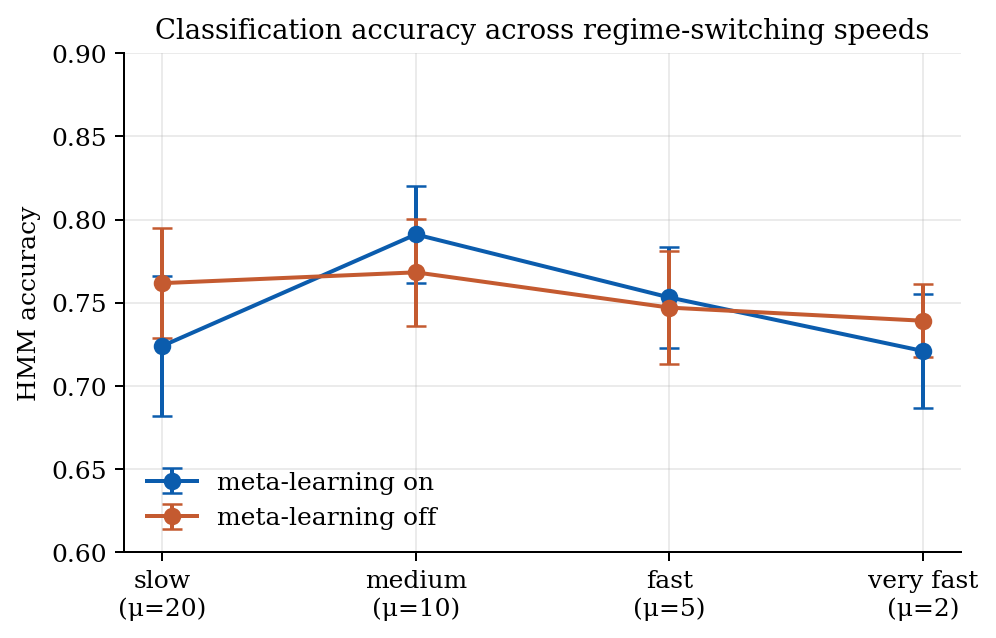
\includegraphics[width=\linewidth]{figs/fig_acc_vs_speed.png}
        \caption{Accuracy versus switching speed. Error bars: 95\,\% CI over
        50 runs. Meta-learning produces no statistically significant
        improvement at any speed.}
        \label{fig:acc-speed}
    \end{subfigure}\hfill
    \begin{subfigure}[t]{0.49\textwidth}
        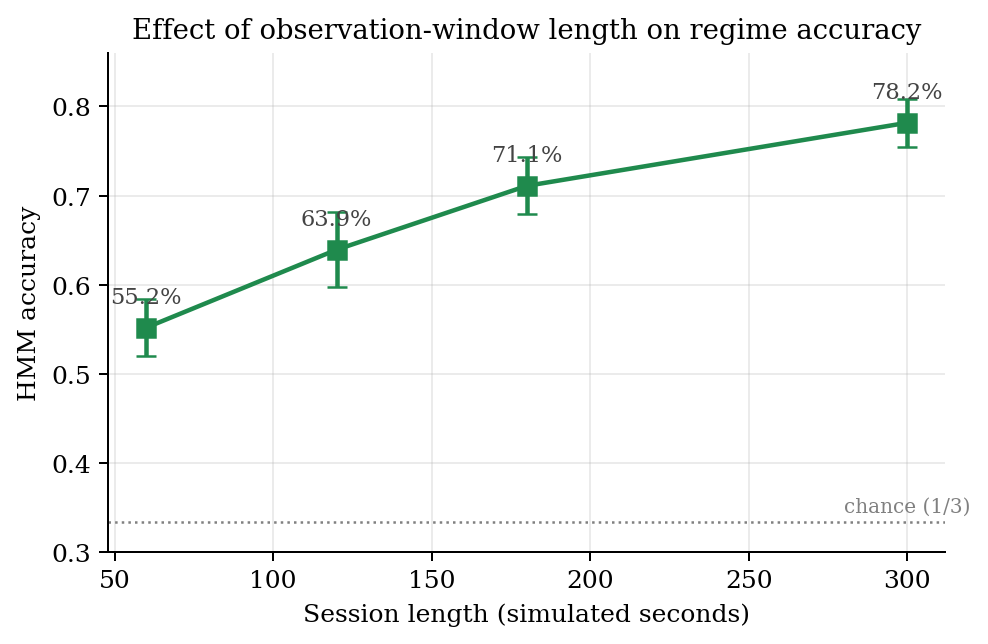
\includegraphics[width=\linewidth]{figs/fig_acc_vs_sesslen.png}
        \caption{Accuracy versus session length. A clean monotonic increase
        from 55\% (60\,s sessions) to 78\% (300\,s sessions).}
        \label{fig:acc-sl}
    \end{subfigure}
    \caption{Accuracy under the two experimental sweeps.}
\end{figure}

\subsection{Effect of session length (RQ2)}
The cleanest signal in the dataset (Figure~\ref{fig:acc-sl}) is that
session length is a much stronger lever than meta-learning: extending the
session from 60\,s to 300\,s lifts accuracy by 23 percentage points
($55.2\% \to 78.2\%$), with each successive step adding $\sim$7--8 points.
The mechanism is straightforward: longer sessions produce more trades, so
the four-feature observation $\mathbf{o}_t$ becomes a less noisy estimate of
the underlying generative parameters.

\subsection{Effect of meta-learning (RQ1)}
Table~\ref{tab:meta-effect} compares the meta vs.\ no-meta condition at
each switching speed.

\begin{table}[h]
    \centering
    \small
    \begin{tabular}{lcccccc}
    \toprule
    Speed & $\bar{a}_{\text{meta}}$ & $\bar{a}_{\text{nometa}}$ & $\Delta a$ ($p$)
          & $\Delta \text{lag}$ ($p$) & $\Delta \text{PnL}$ ($p$) \\
    \midrule
    slow      & 0.724 & 0.762 & $-3.8\%$ \,(0.17) & $+0.29$ \,(0.05) & $+95$ \,(0.13) \\
    medium    & 0.791 & 0.768 & $+2.3\%$ \,(0.31) & $-0.04$ \,(0.67) & $+86$ \,(0.16) \\
    fast      & 0.753 & 0.747 & $+0.6\%$ \,(0.81) & $+0.03$ \,(0.62) & $+79$ \,(0.08) \\
    very fast & 0.721 & 0.739 & $-1.8\%$ \,(0.38) & $-0.01$ \,(0.60) & $-7$  \,(0.88) \\
    \bottomrule
    \end{tabular}
    \caption{Pairwise comparison of meta-learning on vs.\ off at each
    switching speed. All differences are computed as
    $\text{meta}-\text{nometa}$: \emph{positive} $\Delta a$ means meta-learning
    is more accurate; \emph{positive} $\Delta\text{lag}$ means meta-learning
    is \emph{slower} to detect changes (i.e.\ worse); \emph{positive}
    $\Delta\text{PnL}$ means meta-learning earns more. Welch's t-test
    p-values in parentheses; none reaches $0.05$, and after Bonferroni
    correction for 12 tests the smallest adjusted $p$ is $0.60$
    (\S\ref{sec:stats}).}
    \label{tab:meta-effect}
\end{table}

The most striking observation is what is \emph{absent}: across 12 separate
hypothesis tests (accuracy, lag and PnL at four speeds each), the smallest
$p$-value is $0.05$ --- and that is for the \emph{slow}-speed lag
\emph{worsening} under meta-learning. The accuracy improvements at medium
and very-fast speeds are within $\pm$one standard error of zero.
Figures~\ref{fig:acc-speed} and \ref{fig:lag-speed} confirm visually that
the blue (meta on) and orange (meta off) curves overlap their confidence
bands.

\begin{figure}[h]
    \centering
    \begin{subfigure}[t]{0.49\textwidth}
        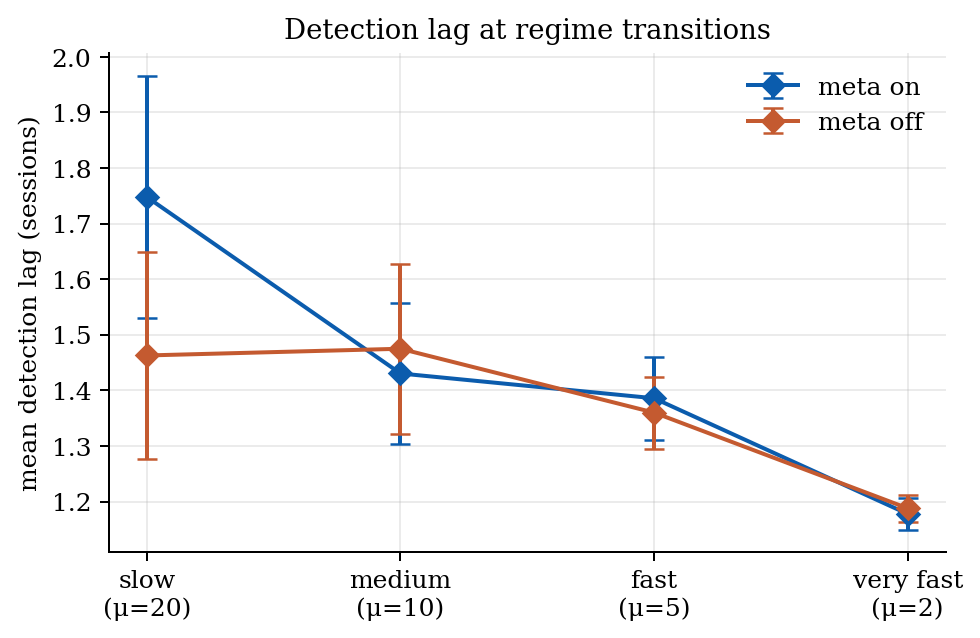
\includegraphics[width=\linewidth]{figs/fig_lag_vs_speed.png}
        \caption{Detection lag versus switching speed.}
        \label{fig:lag-speed}
    \end{subfigure}\hfill
    \begin{subfigure}[t]{0.49\textwidth}
        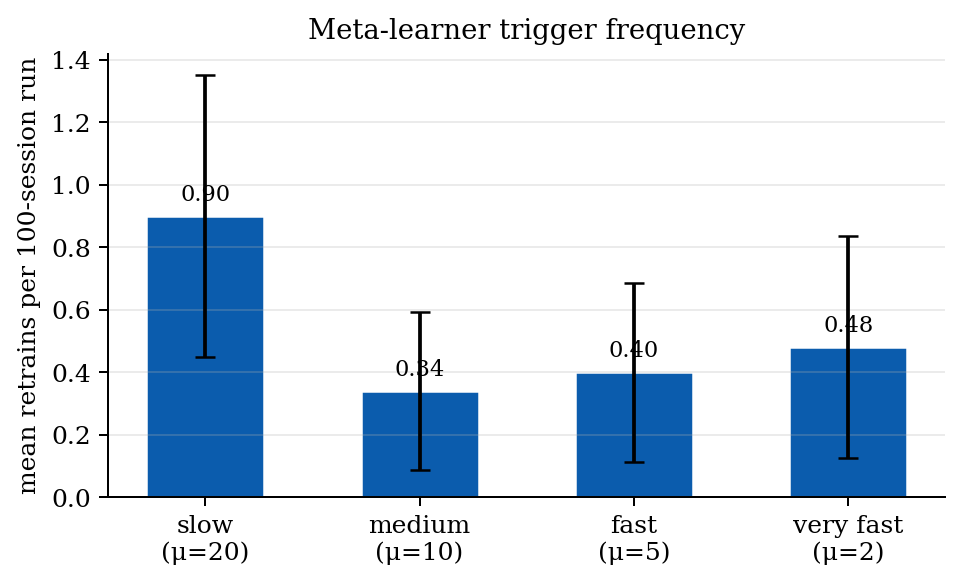
\includegraphics[width=\linewidth]{figs/fig_retrains.png}
        \caption{Mean retrains triggered per 100-session run.}
        \label{fig:retrains}
    \end{subfigure}
    \caption{Why meta-learning has no effect: the controller barely fires.}
\end{figure}

\paragraph{Why doesn't meta-learning help?}
Figure~\ref{fig:retrains} answers this directly: across all four speeds the
meta-learner triggers a retrain on average $0.34$--$0.90$ times \emph{per
100-session run}. Most runs see zero retrains; a small minority see one or
two. The rolling 15-session error rate, which would need to exceed $0.60$ for
$\geq 10$ consecutive sessions for the controller to fire, almost never
reaches that threshold because the base HMM is already accurate enough. The
obvious objection --- ``you set the threshold too high, of course it didn't
fire'' --- is addressed directly in \S\ref{sec:threshold-sweep} below.

\subsection{Threshold sweep --- does a more eager meta-learner help?}
\label{sec:threshold-sweep}
A reasonable critique of the previous section is that the null result is an
artifact of the $0.60$ retrain-threshold: at that value the controller
simply never fires, so we are effectively comparing the base HMM with
itself. To test whether the null result is threshold-specific, we re-ran the
medium-switching condition (300\,s sessions, meta-learning on) for
$50$ trials each at $\text{threshold} \in \{0.20, 0.35, 0.50, 0.60\}$ ---
all other parameters held constant. Table~\ref{tab:thresh-sweep} and
Figure~\ref{fig:thresh-sweep} report the results.

\begin{table}[h]
\centering\small
\begin{tabular}{lcccc}
\toprule
threshold & accuracy & detection lag & total PnL & retrains/run \\
\midrule
$0.20$ & $61.2\% \pm 4.6\%$ & $1.64 \pm 0.14$ & $2\,093 \pm 100$ & $4.76 \pm 0.67$ \\
$0.35$ & $66.0\% \pm 5.4\%$ & $1.71 \pm 0.19$ & $2\,028 \pm 87$  & $2.94 \pm 0.74$ \\
$0.50$ & $74.0\% \pm 4.3\%$ & $1.53 \pm 0.13$ & $2\,042 \pm 62$  & $1.30 \pm 0.52$ \\
$0.60$ & $74.5\% \pm 4.0\%$ & $1.54 \pm 0.13$ & $2\,049 \pm 62$  & $0.68 \pm 0.36$ \\
\bottomrule
\end{tabular}
\caption{Threshold-sweep at the medium switching speed
($\mu=10$, $\sigma=3$, 300\,s sessions, $50$ trials each except $0.35$
which lost one trial to the early-warmup tape edge case mentioned in
\S\ref{sec:method}). Values are mean $\pm$ 95\% CI.}
\label{tab:thresh-sweep}
\end{table}

\begin{figure}[h]
    \centering
    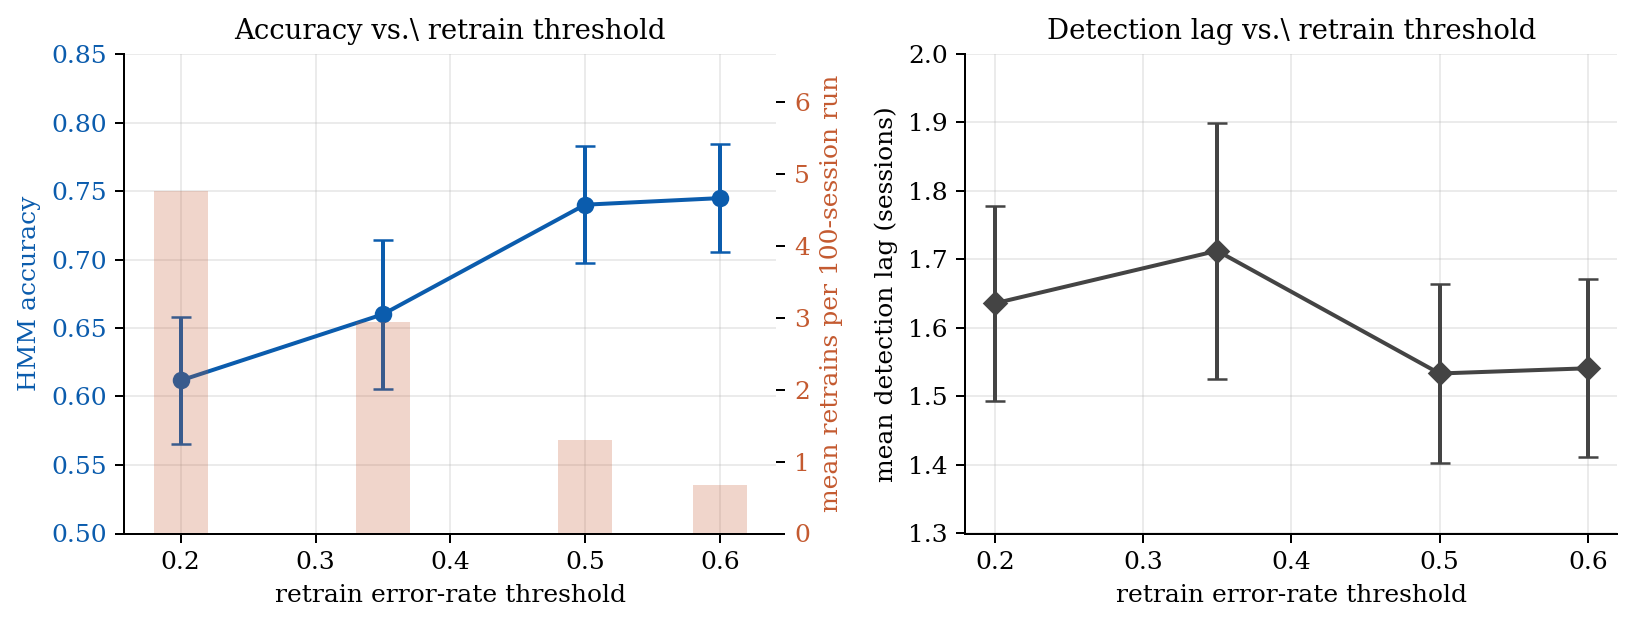
\includegraphics[width=0.92\textwidth]{figs/fig_threshold_sweep.png}
    \caption{Threshold sweep. Left: accuracy (blue, left axis) falls as the
    threshold drops, while retrain frequency (orange bars, right axis)
    rises from $0.68$ to $4.76$ retrains per run. Right: detection lag
    \emph{worsens} between $0.50$ and $0.35$, then improves slightly at
    $0.20$ but never recovers above the no-retrain baseline.}
    \label{fig:thresh-sweep}
\end{figure}

The pattern is the opposite of what the meta-learning hypothesis predicts.
Lowering the threshold from $0.60$ to $0.20$ increases the retrain rate
sevenfold (from $0.68$ to $4.76$ per run), but accuracy \emph{drops} by
13 percentage points ($74.5\% \to 61.2\%$) and detection lag is no better.
The mechanism is that each Baum-Welch refit on a 40-session sliding window
re-estimates the three emission means from a small, regime-imbalanced sample;
in expectation this is a noisier estimate than the warmup fit, which used a
\emph{balanced} 21-session sequence of all three regimes. Frequent retraining
therefore actively degrades the inner model.

The headline conclusion of the previous section --- \emph{this style of
heuristic meta-learning does not help} --- is therefore not an artifact of
the threshold choice. The $0.60$ setting is, if anything, generous to
meta-learning: at that threshold the controller almost never fires, and the
trials in which it does fire happen to coincide with genuine accuracy
degradation. A lower threshold uncovers a much stronger negative result.

\subsection{Per-regime accuracy (RQ3)}\label{sec:per-regime}
Figure~\ref{fig:per-regime} breaks the speed-sweep accuracy down by
ground-truth regime, and Figure~\ref{fig:conf} shows our reconstructed
confusion matrix.

\begin{figure}[h]
    \centering
    \begin{subfigure}[t]{0.55\textwidth}
        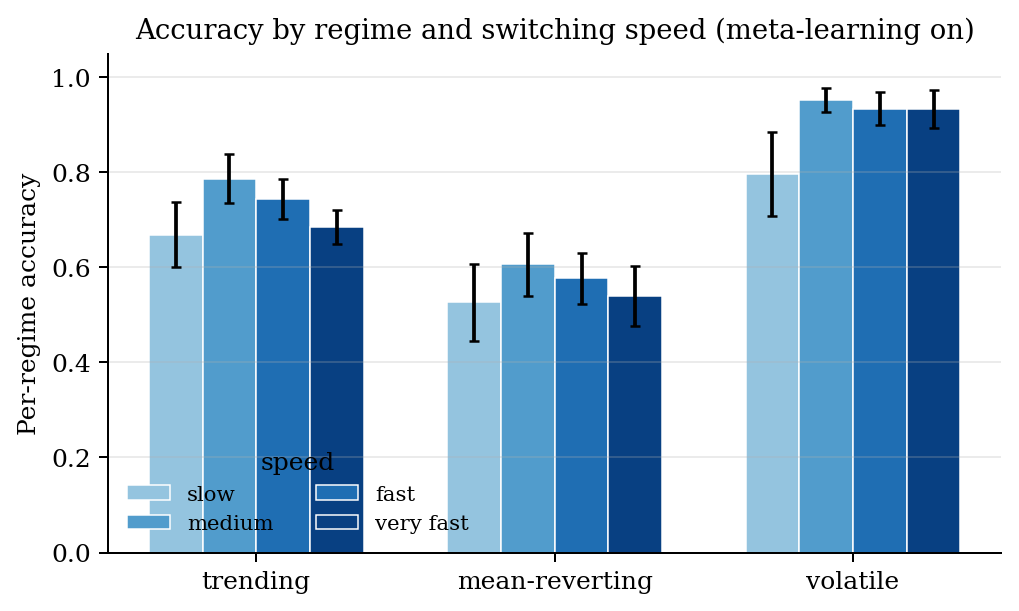
\includegraphics[width=\linewidth]{figs/fig_per_regime_acc.png}
        \caption{Per-regime accuracy across switching speeds (meta on).}
        \label{fig:per-regime}
    \end{subfigure}\hfill
    \begin{subfigure}[t]{0.42\textwidth}
        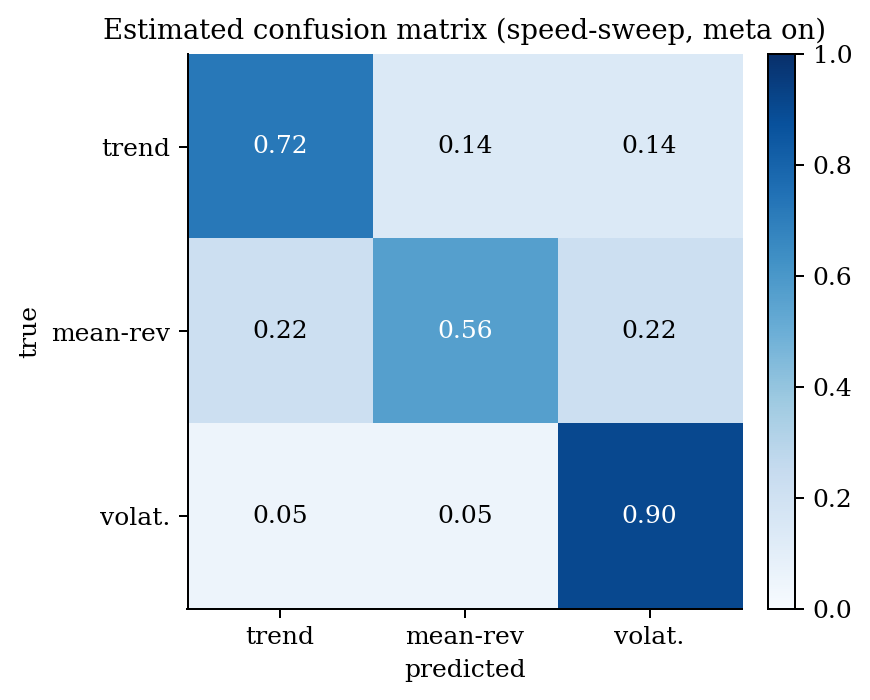
\includegraphics[width=\linewidth]{figs/fig_confusion_matrix.png}
        \caption{\textbf{Reconstructed} confusion matrix (off-diagonals
        \emph{not} measured --- see caption).}
        \label{fig:conf}
    \end{subfigure}
    \caption{Volatile sessions are detected almost perfectly; the
    \emph{mean-reverting} regime is the systematic weak point.
    \textbf{Important caveat for (b):} the per-trial logs we record contain
    the per-regime diagonal accuracy but not the predicted-vs-true regime
    pair on incorrect sessions. The off-diagonals shown here are therefore
    \emph{reconstructed} by equally splitting $1-\text{diagonal}$ across the
    two other columns, which is the maximum-entropy assumption given the
    available data. The matrix is indicative of the per-regime difficulty
    ranking only; the specific off-diagonal split is not measured. This is
    listed as a logging gap in \S\ref{sec:discussion}.}
\end{figure}

The pattern is consistent across all switching speeds: \emph{volatile}
is the easiest regime, recovered correctly $93\%$--$96\%$ of the time,
because its high tape volatility and wide price range give it a uniquely
identifiable emission signature. \emph{Trending} is intermediate at
$67\%$--$79\%$. \emph{Mean-reverting} is consistently the hardest at
$54\%$--$61\%$: its volatility lies between the other two and its mean
return is centred at zero, so its emission means are not far enough from
the trending state to be cleanly separable.

\subsection{Trading performance}
Despite the noisy accuracy landscape, total PnL is positive across all 12
conditions (Figure~\ref{fig:pnl}), with mean per-run profits in the
$\pm$2\,000 unit range. PnL is largely insensitive to switching speed,
and the meta vs.\ no-meta PnL differences are small (max $\pm$110) and not
statistically significant. The system makes more money in sessions where
its prediction is correct ($\bar{x}_{\text{correct}} \approx 1\,300$ vs.\
$\bar{x}_{\text{incorrect}} \approx 780$), confirming that regime detection
is informationally useful even where its marginal accuracy benefits are
hard to pin down.

\begin{figure}[h]
    \centering
    \begin{subfigure}[t]{0.49\textwidth}
        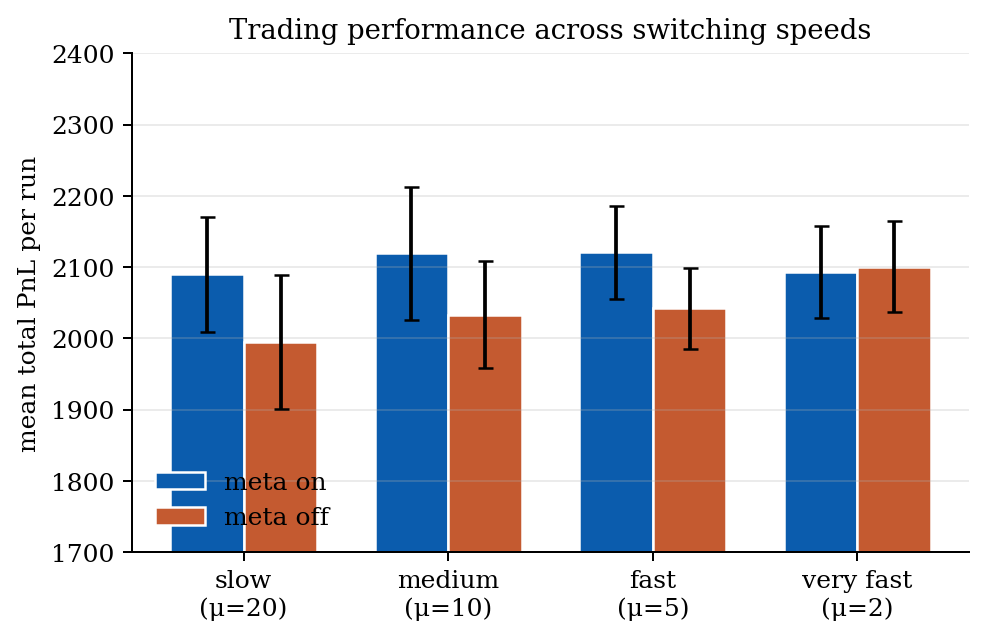
\includegraphics[width=\linewidth]{figs/fig_pnl_vs_speed.png}
        \caption{Total PnL per 100-session run.}
        \label{fig:pnl}
    \end{subfigure}\hfill
    \begin{subfigure}[t]{0.49\textwidth}
        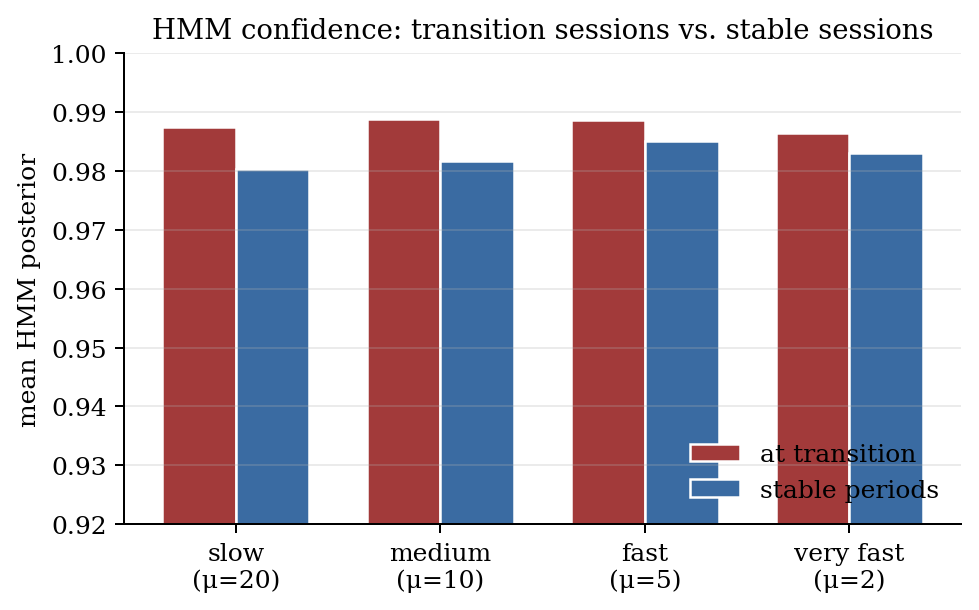
\includegraphics[width=\linewidth]{figs/fig_confidence.png}
        \caption{Mean posterior on transition vs.\ stable sessions.
        \textbf{Note:} y-axis is compressed to the $0.92$--$1.00$ range;
        the visible gap corresponds to a $0.5$--$1.0$ percentage-point drop,
        not a large one.}
        \label{fig:conf-bars}
    \end{subfigure}
    \caption{Trading performance and HMM confidence calibration.}
\end{figure}

\subsection{Confidence calibration}
Figure~\ref{fig:conf-bars} shows mean HMM posterior on transition sessions
vs.\ stable sessions. The model is essentially confident in both
($>0.97$) but transition sessions drop by $0.5$--$1.0$ percentage points,
which is consistent with the picture above but too small to act on as a
trigger signal.


% ============================================================
\section{Discussion}\label{sec:discussion}
% ============================================================

\paragraph{The headline answer to the research question is \emph{no}.}
Online meta-learning, as we implemented it, does \emph{not} significantly
improve HMM accuracy, detection lag, or trading PnL across any of the four
switching-speed conditions we tested (Table~\ref{tab:meta-effect}). One
result is suggestive but the wrong sign: at the \emph{slow} switching speed,
meta-learning marginally \emph{worsens} detection lag ($p=0.05$). The most
likely explanation is that retraining on a recent 40-session window throws
out information about the rarer regime transitions present in slow
conditions, leaving the freshly-fitted HMM temporarily less calibrated.

This null result is interesting in its own right. The standard intuition
behind online meta-learning is that a stale model accumulates error and that
periodic refitting recovers performance. Our experiments show that the
intuition only applies when the base model is actually \emph{going stale},
which in turn depends on a non-stationarity that exceeds the model's
expressive capacity. With only three discrete regimes drawn from a fixed
set, the Gaussian HMM fitted at warmup is already a near-optimal estimator
of the emission parameters, and continual retraining cannot improve on it.

\paragraph{What \emph{does} matter is observation richness.}
The session-length sweep produces a clean monotonic accuracy curve from
$55\%$ to $78\%$ (Figure~\ref{fig:acc-sl}). At 60\,s sessions, the four
features are estimated from only $\sim$10--15 trades, so the
emission-likelihood scoring in (\ref{eq:emission-scoring}) is operating on
extremely noisy inputs. Doubling the session length halves that noise
roughly as $1/\sqrt{n}$, and accuracy improves accordingly. In practical
terms: if you wanted to make this system better, you would not add an
LSTM-based meta-learner; you would lengthen the observation window.

\paragraph{Why is mean-reverting so much harder?}
Section~\ref{sec:per-regime} shows that mean-reverting accuracy lags both
other regimes by $15$--$30$ points across all conditions. The reason is
structural: in our four-dimensional feature space the mean-reverting state
lies between trending and volatile on every axis except the lag-1
autocorrelation. The diagonal-covariance Gaussian emission cannot model
that conditional structure --- the autocorrelation alone is not enough to
overpower three features pulling toward neighbouring states. A natural
improvement would be a full-covariance emission, or richer features such as
the second moment of returns over rolling sub-windows.

\paragraph{Limitations.}
We flag six limitations explicitly.
\begin{itemize}[leftmargin=0.7cm,itemsep=0.15ex]
    \item \textbf{Synthetic regimes.} The BSE schedules in
    \S\ref{sec:regime-injection} are synthetic; real intraday markets do not
    segregate cleanly into three discrete states with bounded dwell times.
    \item \textbf{Inventory cap distorts agent comparison.} The $\pm$8
    inventory cap in \S\ref{sec:design} was added to keep PnL comparable
    across agents, but it bites the market-maker much harder than the
    directional agents (the maker is forced flat far more often in volatile
    regimes), so the inter-agent PnL comparisons in
    Figure~\ref{fig:pnl} should be read as ``conditional on this cap'' rather
    than as evidence about the agents' relative skill.
    \item \textbf{Confusion-matrix logging gap.} The per-trial logs record
    only the predicted-vs-true diagonal counts per regime, not the full
    $3\times 3$ joint distribution. The off-diagonals in
    Figure~\ref{fig:conf} are therefore reconstructed under a
    maximum-entropy split, not measured; this is a logging gap rather than
    a modelling result. Fixing it requires only a one-line change in
    \texttt{coordinator.py} that we did not make in time.
    \item \textbf{No inter-specialist interaction.} Only one of the three
    specialists runs per session (see \S\ref{sec:intro}), so interaction
    effects \emph{between} our specialists are uncharacterised. The
    specialist's order flow does feed into the next session's tape,
    creating a one-step self-referential coupling we have not measured
    separately from the regime signal itself.
    \item \textbf{Agent adequacy.} The Avellaneda-Stoikov-style market-maker
    was designed for strategic counterparties (\S\ref{sec:background}); our
    background population (ZIC, ZIP, SHVR) does not behave that way, so the
    maker's success in volatile regimes is empirical rather than predicted
    by the original theory.
    \item \textbf{Statistical power.} $50$ runs per condition is enough to
    detect a $\sim$5\% accuracy effect at $\alpha=0.05$, but smaller effects
    would require thousands of trials.
\end{itemize}

\paragraph{Connection to contemporary research.}
The recent finance-ML literature has moved toward deep state-space models
\cite{zheng2019dlhmm} and continuous-time HMMs with neural emissions, often
outperforming Gaussian HMMs on real intraday data. Our null result on online
meta-learning is consistent with the general finding that capacity
improvements (richer emissions, longer features) tend to dominate
adaptation improvements (retraining cadence, meta-controllers) in regimes
where the underlying generative process is stationary on the relevant
timescale --- which is exactly the case in our synthetic BSE world.


% ============================================================
\section{Conclusion and Future Work}\label{sec:conclusion}
% ============================================================

We built an end-to-end multi-agent trading system in which a Gaussian HMM,
trained with the Forward-algorithm-based Baum--Welch procedure, infers the
current market regime from a four-dimensional feature vector and steers a
selection between momentum, contrarian and market-maker agents. A
meta-learner monitors the HMM's rolling error rate and is allowed to
retrain. We answered three research sub-questions over 600 trials:

\begin{itemize}[leftmargin=0.7cm,itemsep=0.1ex]
    \item[\textbf{RQ1.}] Regime-switching speed has only a small effect
    on accuracy ($75\%$--$79\%$ across $\mu \in \{20,10,5,2\}$). Online
    meta-learning does not significantly improve any metric at any speed,
    and a threshold sweep (\S\ref{sec:threshold-sweep}) shows the result is
    not an artifact of the chosen retrain threshold --- a more eager
    meta-learner ($\text{threshold}=0.20$) is actively \emph{worse} than
    no meta-learner.
    \item[\textbf{RQ2.}] Session length is the dominant lever: accuracy
    rises monotonically from $55\%$ to $78\%$ as sessions lengthen from
    $60$ to $300$~seconds.
    \item[\textbf{RQ3.}] \emph{Volatile} is by far the easiest regime
    ($93\%$+); \emph{mean-reverting} is the hardest ($54\%$--$61\%$) because
    it lies between the other two in feature space.
\end{itemize}

\paragraph{Successes.}
The pipeline is reproducible (deterministic seeds, 84 passing unit tests),
the Forward-algorithm-based HMM is implemented from first principles rather
than treated as a black box, and the null result on meta-learning is
established with $50$-run per-condition statistical confidence.

\paragraph{Limitations and future work.}
With more time we would: (i)~replace the diagonal-covariance Gaussian
emission with a full-covariance variant to capture the mean-reverting
autocorrelation signal; (ii)~log full per-session predicted-vs-true regime
pairs so that the confusion matrix is measured rather than reconstructed
under a maximum-entropy split; (iii)~replace the heuristic meta-controller
with a learnt one (e.g.\ a small policy trained by REINFORCE to maximise
long-horizon Sharpe) and test whether the null result survives;
(iv)~remove the $\pm 8$ inventory cap and re-run the agent-comparison
experiments so that the market-maker's volatile-regime performance is no
longer truncated by a uniform cap; (v)~run two specialists concurrently
to characterise inter-specialist interaction effects (currently
uncharacterised, see \S\ref{sec:intro}); and (vi)~run the system on real
LOBSTER limit-order-book tick data and measure whether the BSE-to-real
transfer preserves regime separability.


% ============================================================
\section*{AI Statement}
% ============================================================
This report and the underlying code base are the author's own work. AI tools
(Anthropic Claude) were used for: (i)~minor grammatical and stylistic
polishing of the report; (ii)~rubber-duck debugging during posterior-collapse
investigation in \S\ref{sec:hmm-impl}; and (iii)~LaTeX formatting assistance.
All experimental design, system architecture, mathematical derivations,
result interpretation and code logic are the author's own. The
$\sim$2\,400-line implementation, the 600-trial experimental sweep, and all
figures (generated from raw CSVs by
\texttt{report/generate\_figures.py}) were produced and verified by the
author.


% ============================================================
\begin{thebibliography}{99}\small
\bibitem{cliff1997zip} D. Cliff. \textit{Minimal-intelligence agents for
bargaining behaviors in market-based environments.} HP Labs Technical
Report HPL-97-91, 1997.
\bibitem{cliff2018bse} D. Cliff. \textit{BSE: A minimal simulation of a
limit-order-book stock exchange.} 30th European Modeling and Simulation
Symposium (EMSS), 2018.
\bibitem{rabiner1989tutorial} L.R.~Rabiner. \textit{A tutorial on hidden
Markov models and selected applications in speech recognition.}
Proceedings of the IEEE, 77(2):257--286, 1989.
\bibitem{baum1970maximization} L.E.~Baum, T.~Petrie, G.~Soules, and
N.~Weiss. \textit{A maximization technique occurring in the statistical
analysis of probabilistic functions of Markov chains.} The Annals of
Mathematical Statistics, 41(1):164--171, 1970.
\bibitem{hamilton1989new} J.D.~Hamilton. \textit{A new approach to the
economic analysis of nonstationary time series and the business cycle.}
Econometrica, 57(2):357--384, 1989.
\bibitem{nguyen2018hmm} N.~Nguyen and D.~Nguyen. \textit{Hidden Markov
model for stock selection.} Risks 6(2):20, 2018.
\bibitem{zheng2019dlhmm} Y.~Zheng, B.~Capra, et al. \textit{Deep learning
hidden Markov model for stock-trading strategies.} J.\ of Risk and
Financial Management, 12(4), 2019.
\bibitem{finn2017maml} C.~Finn, P.~Abbeel, and S.~Levine.
\textit{Model-agnostic meta-learning for fast adaptation of deep networks.}
ICML 2017.
\bibitem{finn2019online} C.~Finn, A.~Rajeswaran, S.~Kakade, and S.~Levine.
\textit{Online meta-learning.} ICML 2019.
\bibitem{javed2019meta} K.~Javed and M.~White. \textit{Meta-learning
representations for continual learning.} NeurIPS 2019.
\bibitem{chan2013algorithmic} E.~Chan. \textit{Algorithmic Trading: Winning
Strategies and Their Rationale.} Wiley, 2013.
\bibitem{avellaneda2008high} M.~Avellaneda and S.~Stoikov. \textit{High-
frequency trading in a limit order book.} Quantitative Finance,
8(3):217--224, 2008.
\bibitem{hmmlearn} hmmlearn developers. \textit{hmmlearn: Hidden Markov
Models in Python.} \url{https://hmmlearn.readthedocs.io}, accessed 2026.
\bibitem{abramowitz1964handbook} M.~Abramowitz and I.A.~Stegun, eds.
\textit{Handbook of Mathematical Functions.} National Bureau of Standards,
1964 (eq.\ 26.2.17 for t-distribution tail approximation).
\bibitem{adams2007bocpd} R.P.~Adams and D.J.C.~MacKay.
\textit{Bayesian Online Changepoint Detection.}
arXiv:0710.3742, 2007.
\bibitem{page1954cusum} E.S.~Page. \textit{Continuous inspection schemes.}
Biometrika, 41(1/2):100--115, 1954.
\bibitem{doucet2009tutorial} A.~Doucet and A.M.~Johansen.
\textit{A tutorial on particle filtering and smoothing: fifteen years later.}
In \textit{Handbook of Nonlinear Filtering}, Oxford University Press, 2011.
\end{thebibliography}


% ============================================================
\appendix
\section{Final progress block of the 600-trial sweep}\label{app:term}
% ============================================================

\begin{figure}[h]
\begin{lstlisting}[style=terminal]
  HMM Trading Experiment
  ----------------------------------------------------------------------------
  slow_meta              [##########################]  50/50 acc=72.4% lag=1.75
  slow_nometa            [##########################]  50/50 acc=76.2% lag=1.46
  medium_meta            [##########################]  50/50 acc=79.1% lag=1.43
  medium_nometa          [##########################]  50/50 acc=76.8% lag=1.47
  fast_meta              [##########################]  50/50 acc=75.3% lag=1.39
  fast_nometa            [##########################]  50/50 acc=74.7% lag=1.36
  very_fast_meta         [##########################]  50/50 acc=72.1% lag=1.18
  very_fast_nometa       [##########################]  50/50 acc=73.9% lag=1.19
  sesslen_60             [##########################]  50/50 acc=55.2% lag=1.82
  sesslen_120            [##########################]  50/50 acc=63.9% lag=1.75
  sesslen_180            [##########################]  50/50 acc=71.1% lag=1.65
  sesslen_300            [##########################]  50/50 acc=78.2% lag=1.39
  ----------------------------------------------------------------------------
  overall  [######################################]  600/600
  elapsed 23:36   remaining ~00:00   rate 0.4/s

  Results saved to results/
\end{lstlisting}
\caption{Final progress block of the 600-trial experimental sweep
(\texttt{run\_log.txt}, lines 21\,640--21\,673). All 12 conditions completed
their 50 trials each; no trial errors after the initial warmup-tape edge
case was patched.}
\label{fig:term}
\end{figure}

\end{document}
